\documentclass{article} \usepackage{amsmath} \usepackage{amssymb} \usepackage{amsthm} \usepackage[margin=0.2in]{geometry} \usepackage{hyperref} \usepackage{physics} \usepackage{tikz} \usepackage{mathtools} \mathtoolsset{showonlyrefs} \theoremstyle{definition} \newtheorem{theorem}{Theorem}[section] \newtheorem{corollary}{Corollary}[theorem] \newtheorem{lemma}[theorem]{Lemma} \newtheorem{definition}{Definition}[section] \author{Connor Duncan} \date{\today}
\title{Physics-105-Lecture-Notes-03-05-2019}
\begin{document}
\maketitle\tableofcontents
\noindent\abstract{A single PDF with all lectures in a single document can be downloaded at \url{https://www.dropbox.com/sh/8sqzvxghvbjifco/AAC9LoSRnsRQDp7pYedgWpQMa?dl=0}. The password is 'analytic.mech.dsp'.
 This file was automatically generated using a script, so there might be some errors. If there are, you can contact me at \url{mailto:ctdunc@berkeley.edu}.}
Energy diagram, recall from previous week where the minimum with one $r$ is a circular orbit, i.e. $\dv{V}{r_0}=0$, question is only whether or not its stable, i.e. a relative minimum or maximum. there was already a homework problem on this, so I would watch out if I were you! \subsection{Ex: find stable circular orbits (this is very similar to the homework!)} $F(r)=\frac{-k}{r^n}$, which gives $V(r)=\frac{k}{(n-1)r^{n-1}}$, with effective potential $V_e(r)=\frac{l^2}{2mr^2}-\frac{k}{(n)r^{n-1}}$. Stable point of this? $\dv{V}{r}=\frac{k}{r^n}-\frac{l^2}{mr^3}=0$ which gives $r_0=\left(\frac{mk}{l^2}\right)^{-n+3}$. So, for stable orbits, $\dv{V}{r}=\frac{-nk}{r^{n+1}}+\frac{3l^2}{mr^4}>0$, which gives $(3-n)\frac{l^2}{m}>0$ which implies that $n<3$ must be the case for stable circular orbits. If we want pertubations around a stable orbit, we can taylor expand aroudn the equilibrium point ($r_0$). We have the equation of motion \begin{equation} m\ddot r-\frac{l^2}{mr^2}=-f(x)=-\dv{L}{r} \end{equation} At this point, bale kind of gave up because he doesn't want to give away the answer to the homework, but hit me up if u have any questions, the algebra SUCKS. \section{Hamiltonian Mechanics} \subsection{Rutherford Scattering} We're talking about quantum mechanics rn, because the hamiltonian is very imortant. Rutheford scattering, observed really large alpha particle scattering which was weird. \begin{center} 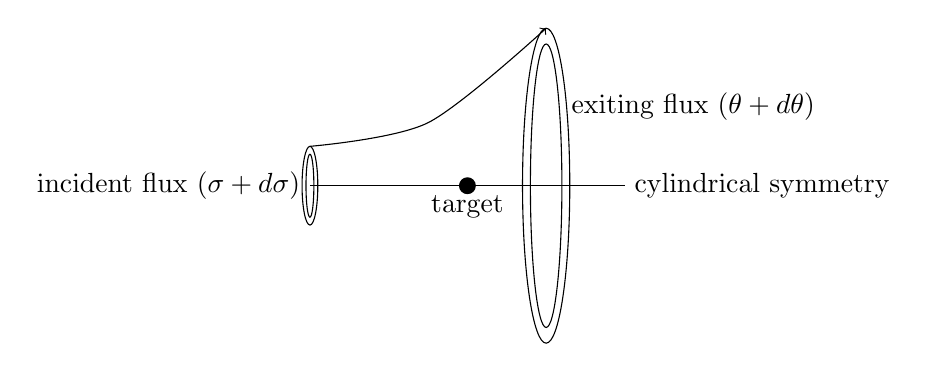
\begin{tikzpicture} \draw[->] plot [smooth] coordinates {(-2,0.5)(-0.5,0.8)(1,2)}; \draw (-2,0)--(2,0) node[anchor=west]{cylindrical symmetry}; \draw[fill] (0,0) ellipse (0.1) node[anchor=north]{target}; \draw (-2,0) ellipse (0.1 and 0.5) (-2,0) ellipse (0.05 and 0.4) node[anchor=east]{incident flux $(\sigma+d\sigma)$}; \draw (1,0) ellipse (0.3 and 2) (1,0) ellipse (0.2 and 1.8) (1.2,1)node[anchor=west]{exiting flux ($\theta+d\theta$)}; \end{tikzpicture} \end{center} Some differential cross section of the angle between the horizontal and scattering at infinity is given as \begin{equation} d\sigma(\text{into}d\Omega)=\frac{d\sigma}{d\Omega}d\Omega \end{equation} by into $d\Omega$ I have no idea what he measn yet. It will become clear. \begin{equation} \sigma=\int\frac{d\sigma}{d\Omega}d\Omega=\int_0^\pi\sin\theta d\theta\int_0^{2\pi}d\varphi\frac{d\sigma }{d\Omega}(\theta,\varphi) \end{equation} we could try doing this with conservation of angular momentum, that $l=mv_0s$. Or, take the total energy $E=\frac{1}{2}mv_0^2$ where $v_0$ in both represents the velocity at $r=-\infty$. Eliminating $v_0$, we have $l=\sqrt{2mE}$. Integrating this for the impluse, we get \begin{equation} \Psi =\int_{r_1}^{\infty}\frac{dr}{r^2\sqrt{\frac{2mE}{l^2}+\frac{2mV(r)}{l^2}-\frac{1}{r^2}}} \end{equation} We can just cut to the chase, and say there's a hyperbolic orbit with central forcing, of which we already have an equation (doesn't this picture look kind of familiar?). \begin{equation} k=-z_1z_2e^2 \end{equation} deno ting coulomb force, then we can write (double check this in the book, I was way too far away to see this coherently) \begin{equation} \frac{1}{r}=-\frac{mz_1z_2e^2}{l^2}(1+\epsilon\cos\psi) \end{equation} So, as $r\rightarrow\infty$, we have $\frac{1}{r}\rightarrow 0=\frac{mz_1z_2e^2}{l^2}(\epsilon\cos\psi+1)$. This gives that \begin{equation} \cos^2\frac{\theta}{2}=\frac{\epsilon^2-1}{\epsilon^2} \end{equation} which gives \begin{equation} \cot^2\frac{\theta}{2}=\epsilon^2-1=\frac{2Es}{z_1z_2e^2} \end{equation} Now, we have a solution for $s$, \begin{equation} s=\frac{z_1z_2e^2}{2E}\cot^2\frac{\theta}{2} \end{equation} which gives \begin{equation} \sigma(\theta)=\frac{1}{4}\left(\frac{z_1z_2e^2}{2E}\right)^2\csc^4\frac{\theta}{2}=\frac{s}{\sin\theta}\dv{s}{\theta} \end{equation} This was a super messy derivation of this idea, so I would probably look it up/check back into a textbook for a better idea, especially because notation wasn't super consistent/things were p hard to see. \subsection{Beginning Hamiltonian Mechanics} Recall we defined $\mathcal{L}(q,\dot q,t)=T-V$, with the appropriate euler lagrange equations. We also defined generalized momentum, $p=\pdv{\mathcal L}{\dot q}$. The hamiltonian formulation takes out the $\dot q$ dependence and replaces it with $p$. \begin{equation}\label{eqdef:hamiltonian} H=\sum_ip_i\dot q_i-\mathcal{L}(q,\dot q(q,p),t)=H(q,p,t) \end{equation} We're now working in a $2n$ dimensional ``phase space'' $(p,q)$. Dropping $i$', we have \begin{align} \pdv{H}{p}=\pdv{}{p}\left(\sum_ip_i\dot q_i-\mathcal{L}(q,\dot q(q,p),t)\right)\\ =\dot q+p\pdv{\dot q}{p}-\pdv{\mathcal L}{\dot q}\pdv{\dot q}{p}\\ =\dot q\\ \pdv{H}{q}=\pdv{}{q}\left(\sum_ip_i\dot q_i-\mathcal{L}(q,\dot q(q,p),t)\right)\\ =p\pdv{\dot q}{q}-\pdv{\mathcal L}{q}-\pdv{\mathcal L}{\dot q}\pdv{\dot q}{q}\\ =-\pdv{\mathcal L}{q} \end{align} which, by the euler-lagrange equations gives \begin{equation} \pdv{H}{q}=-\dv{}{t}\left(\pdv{L}{\dot q}\right)=-\dv{}{t}q \end{equation} Finally, we might also take \begin{align} \pdv{H}{t}=\pdv{}{t}\left(\sum_ip_i\dot q_i-\mathcal{L}(q,\dot q(q,p),t)\right)\\ =p\pdv{\dot q}{t}-\pdv{\mathcal L}{\dot q}... \end{align} he goes too fast lmao. Gives \textbf{Hamiltons Equations of Motion} \begin{align} \dot q=\pdv{H}{p}\\ \dot p=-\pdv{H}{q}\\ \pdv{H}{t}=-\pdv{\mathcal L}{t} \end{align} \subsection{ex: hamiltonian, sho} We can do some fancy algrebra to derive that for a simple harmonic oscillator, we get \begin{equation} H=\frac{p^2}{2m}+\frac{1}{2}kx^2 \end{equation} Note from Connor, ur friendly DSP boi, this is super similar to quantum mechanics hamiltonian! \subsection{ex: Particle, Magnetic field} Trust and verify that the lagrangian is written as \begin{equation} \mathcal L=\frac{1}{2}m\dot r^2-e\varphi(r,t)+\frac{e}{c}\dot{\vec{r}}\cdot\vec{A}(r,t) \end{equation} with $B=\vec{\nabla}\times\vec{A}$, and $\vec{E}=-\vec{\nabla}\varphi-\frac{1}{c}\dv{\vec{A}}{t}$. Basically just do the math out. I swear, I cannot see the board on the other side of the room, so I'll try and do this out on my own, or talk to somebody in the class to get this example. Hamiltons equations of motion: also gives u ray tracing, from optics.
\end{document}
